\section{Geometry}
\subsection{Derivation of the Pin-hole Camera Transformation}
Conventionally, world coordinates are denoted with subscript $w$ and uppercase $\Vect{P}$ to show its unit is [m], $\Vect{P}_w$. Camera coordiantes are $\Vect{P}_c$. In this note, world coordinate  can also be expressed in $\Vect{P}_0$, while camera coordinate in $\Vect{P}_i$, $i\in \bbN^+$.

\begin{figure}[htbp]

\centering

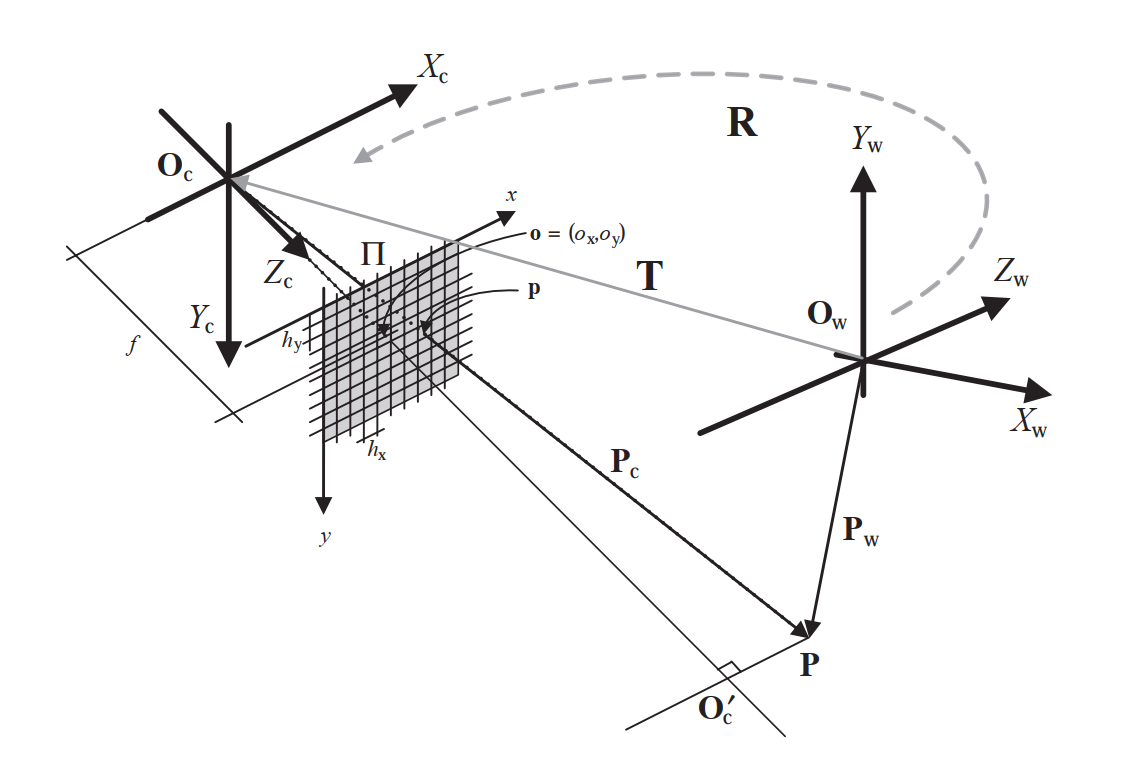
\includegraphics[width=0.7\linewidth]{figure/pin_hole_model.png}

\caption{Pin-hole model of the perspective camera with two coordinate systems: world \textbf{W} and
camera \textbf{C}. Readers need to be careful that the symbol notations  in this figure are not completely consistent with this note. Courtesy of Boguslaw and J. Paul, \textit{An Introduction to 3D Computer Vision Techniques and Algorithms}.}

\end{figure}

\subsubsection{Extrinsic Parameters}
\begin{equation}
\Vect{T}_{wc} = (\overline{\Vect{O}_w \Vect{O}_c})_w,
\end{equation}
\begin{equation}
\Vect{P}_{\mathrm{c}}=\Matr{R}_{wc}  \left(\Vect{P}_{w}-\Vect{T}_{wc}\right)=[x_{c},y_c,z_c]^T,
\end{equation}
whose inverse is easy to get, that is, $\Vect{P}_{w}=\Matr{R}^{T}_{wc} \Vect{P}_{c}+\Vect{T}_{wc}$. Next step, the point $\Vect{P}_c$ is projected onto the image plane by the classic perspective method. 

\begin{definition}
Extrinsic parameters refers the translation vector $\Vect{T}$ and rotation matrix $\Matr{R}$.\\
外参数指的的平移向量 $\Vect{T}$ 和旋转矩阵 $\Matr{R}$,共包含六个独立标量。
\end{definition}

\subsubsection{Intrinsic Parameters}

As part of intermediate step, the projected point is still in the camera coordinate, denoted as $\tilde{\Vect{P}}_c=[f x_c/z_c, f  y_c/z_c, f]$. What's more, the points on image plane may experience a geometric distortions. To recover, a factor $1/(1+k_1 r^2+k_2 r^4)$ is expected.
Values $k_1, k_2$ might be distinct for $x$ and $y$ axis. 

Here are some limitations which restrict an ideal infinite plane. (1) \textbf{Limited sampling area}, (2) \textbf{Invalid region} due to incorrect focus and so on. 


Now one can transform the image plane coordinate to pixel image coordinate $\Vect{p}_c$. 

$$x_p=\frac{f}{h_x} \frac{x_c}{z_c}+o_{px},$$
$$y_p=\frac{f}{h_y} \frac{y_c}{z_c}+o_{py},$$
where $h_x$ usually means how many micrometers per pixel [$\mu$m/pixels]. Subscript $p$ means the quantity has the unit [pixel].

Here is another type of expression (not important enough, just explain it  here) with homogeneous coordiantes $\Vect{p}_{ph}=[x_{ph},y_{ph},z_{ph}]$. The subscript $ph$ means the coordiante is handle from unit [pixel] to be homogeneous with unit [m], it in fact can represent a whole straight line in the camera coordinate.

\begin{equation}
\left\{\begin{array}{l}
	{x_{ph}=\frac{f}{h_{x}} x_c+o_{px} z_c} \\ 
	{y_{ph}=\frac{f}{h_{y}} y_c+o_{py} z_c} \\ 
	{z_{ph}=z_c}
	\end{array}\right.
\end{equation}

\begin{equation}
\Vect{p}_{ph}=\left[\begin{array}{c}{x_{ph}} \\ {y_{ph}} \\ {z_{ph}}\end{array}\right]=\underbrace{\left[\begin{array}{ccc}{\frac{f}{h_{x}}} & {0} & {o_{\mathrm{px}}} \\ {0} & {\frac{f}{h_{y}}} & {o_{\mathrm{py}}} \\ {0} & {0} & {1}\end{array}\right]}_{\Matr{M}_i} \Matr{R}_{wc}  \left(\Vect{P}_{w}-\Vect{T}_{wc}\right)=\left[\begin{array}{ccc}{\frac{f}{h_{x}}} & {0} & {o_{\mathrm{px}}} \\ {0} & {\frac{f}{h_{y}}} & {o_{\mathrm{py}}} \\ {0} & {0} & {1}\end{array}\right] \Vect{P}_c
\end{equation}

\begin{definition}
Intrinsic parameters include:
\begin{enumerate}
	\item Intrinsic matrix, $\Matr{M}_i$, tells the transform rule from camera coordiantes to pixel image coordiantes.
	\item Distortion parameters $k_1$, $k_2$, which is able to recover the distorted image.
	\item Focal length $f_x$, $f_y$. 
\end{enumerate}

内参数指的是
\begin{enumerate}
	\item 内矩阵, $\Matr{M}_i$, 如何将相机坐标转化为像素的图像坐标.
	\item 形变参量 $k_1$, $k_2$, 由于矩阵的鱼眼效应,图像会出现一些变形,这两个参数用于恢复这种变形.
	\item 焦距 $f_x$, $f_y$, x、y 方向上可能有不同. 
\end{enumerate}
\end{definition}

\subsection{Epipolar Geometry, 双目视觉}

\begin{figure}[htbp]

\centering

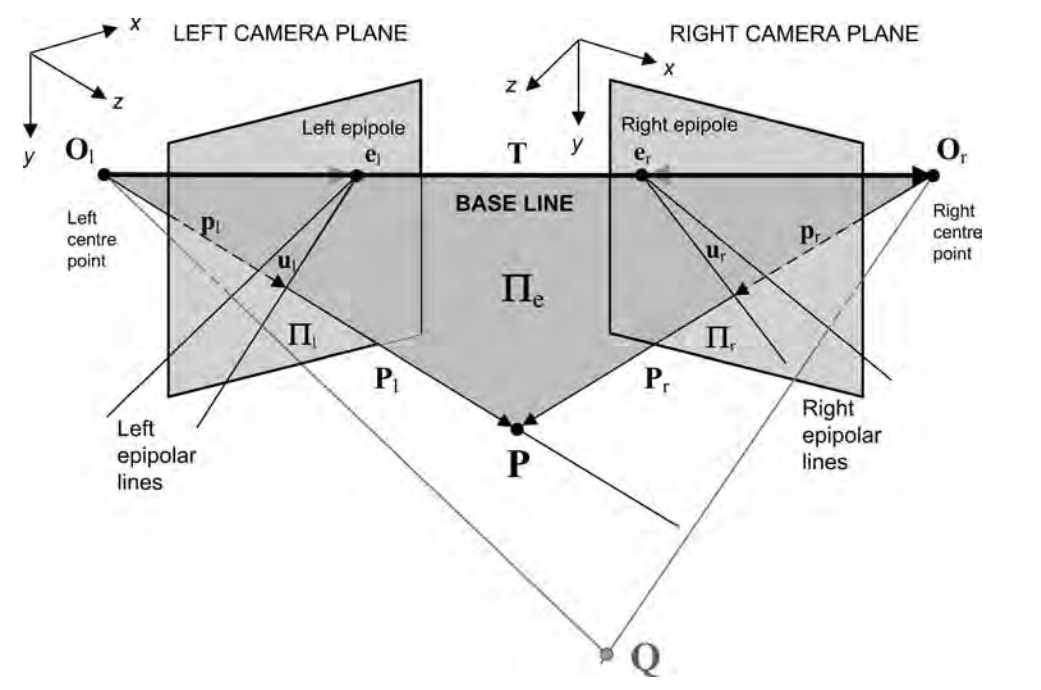
\includegraphics[width=0.7\linewidth]{figure/epipolar_geometry.png}

\caption{Epipolar Geometry. Courtesy of Boguslaw and J. Paul, \textit{An Introduction to 3D Computer Vision Techniques and Algorithms}.}

\end{figure}

\subsubsection{Essential Matrix, $\Matr{E}$ 矩阵}
$$\Vect{P}_2=\Matr{R}_{12}(\Vect{P}_1-\Vect{T}_{12})$$

From the perspective of coordinate 1, $\Vect{P}_1$, $\Vect{T}_{12}$, $\Vect{P}_1-\Vect{T}_{12}$ are in the same plane evidently.
Then we have 

\begin{equation}
\left(\Vect{P}_{1}-\Vect{T}_{12}\right) \cdot\left(\Vect{T}_{12} \times \mathbf{P}_{1}\right)=\left(\Vect{P}_{1}-\Vect{T}_{12}\right) \cdot\left(\Matr{s}(\Vect{T}_{12})  \Vect{P}_{1}\right)=0
\end{equation}

\marginnote{Here we define $\Matr{s}(\Vect{V})$ to map a vector $\Vect{V}$ to a antisymmetric matrix. 
\begin{equation}
\Matr{s}(\Vect{V}) = \begin{bmatrix}0 & -V_3 & V_2 \\V_3 & 0 & -V_1 \\ -V_2 & V_1 & 0 \end{bmatrix}
\end{equation}
}
\begin{equation}
\left(\Matr{R}_{12}^{-1} \Vect{P}_{2}\right)^{T} \Matr{s}(\Vect{T}_{12}) \Vect{P}_{1}=0
\end{equation}


\begin{equation}\label{formula:essential_matrix}
\mathbf{P}_{2}^{\mathrm{T}} \underbrace{\Matr{R}_{12} \Matr{s}(\Vect{T}_{12})}_{\Matr{E}_{12}} \Vect{P}_{1}=0
\end{equation}
\begin{definition}
(\textbf{Essential Matrix})

Chaning coordinate from 1 to 2, essential matrix $\Matr{E}_{12}$ refers to the kernel matrix which vanishes when multiplied by the position vector of the same point in different coordiantes, $\Vect{P}_2^T$ on the left and $\Vect{P}_1$ on the right.

If $\Matr{E}_{12}$ is multiplied by $\Vect{P}_1$ on the right, the left null space of $\Matr{E}_{12}\Vect{P}_1$ indicates the line where the point must locate in the coordinate 2. On the contrary, the right null space of $\Vect{P}_2^T \Matr{E}_{12}$ corresponds to the line in the coordinate 1.

在双目视觉的两个相机坐标系变换过程中, $\Matr{E}_{12}$ 表示的是这么一个核矩阵,它使得 $\Vect{P}$ 点在两个坐标系中的坐标满足下面的关系:
\begin{equation}
	\Vect{P}_2^T\Matr{E}_{12}\Vect{P}_1=0
\end{equation}

进一步剖析,
\begin{itemize}
	\item $\Matr{E}_{12}\Vect{P}_1$ 的零空间,表示在 2 摄影机坐标下,已知$\Vect{P}_1$ 后所确定的 $\Vect{P}$ 点可能所在的直线,
	\item $\Vect{P}_2^T \Matr{E}_{12}$ 的零空间,表示在 1 摄影机坐标下,已知$\Vect{P}_2$ 后所确定的 $\Vect{P}$ 点可能所在的直线,
\end{itemize}


\end{definition}
\subsubsection{Fundamental Matrix, $\Matr{F}$ 矩阵}

Different from the essential matrix, the fundamental matrix directly works on the pixel image coordiantes.

$$\Vect{p}_{1h} = (\Matr{M}_i)_1 \Vect{P}_1$$
$$\Vect{p}_{2h} = (\Matr{M}_i)_2 \Vect{P}_2$$

Substitute the $\Vect{p}_{1h}$, $\Vect{p}_{1h}$ into the equation \ref{formula:essential_matrix}.

\begin{equation}\label{formula:fundamental_matrix}
\mathbf{p}_{2h}^{T} \underbrace{ ((\Matr{M}_{i})_2^{-1})^T \Matr{R}_{12} \Matr{s}(\Vect{T}_{12}) (\Matr{M}_{i})_1^{-1}}_{\Matr{F}_{12}} \Vect{p}_{1h}=0
\end{equation}

\begin{definition}
	(\textbf{Fundamental Matrix})
	
	Chaning pixel image coordiantes from 1 to 2, fundamental matrix $\Matr{F}_{12}$ refers to the kernel matrix which vanishes when multiplied by the homogeneous position vector of the same point in different coordiantes, $\Vect{p}_{2h}^T$ on the left and $\Vect{p}_{1h}$ on the right.
	
	If $\Matr{F}_{12}$ is multiplied by $\Vect{p}_{1h}$ on the right, the left null space of $\Matr{E}_{12}\Vect{p}_{1h}$ indicates the line where the point must locate in the coordinate 2. On the contrary, the right null space of $\Vect{p}_{2h}^T \Matr{E}_{12}$ corresponds to the line in the coordinate 1.

	在双目视觉的两个相机坐标系变换过程中, $\Matr{E}_{12}$ 表示的是这么一个核矩阵,它使得 $\Vect{P}$ 点在两个坐标系中的坐标满足下面的关系:
\begin{equation}
	\Vect{p}_{2h}^T\Matr{F}_{12}\Vect{p}_{1h}=0
\end{equation}

进一步剖析,
\begin{itemize}
	\item $\Matr{F}_{12}\Vect{p}_{1h}$ 的零空间,表示在 2 齐次像坐标下,已知$\Vect{p}_{1h}$ 后所确定的 $\Vect{P}$ 点可能所在的直线,
	\item $\Vect{p}_{2h}^T \Matr{F}_{12}$ 的零空间,表示在 1 齐次像坐标下,已知$\Vect{p}_{2h}$ 后所确定的 $\Vect{P}$ 点可能所在的直线,
\end{itemize}
\end{definition}

\subsection{Constraints}
Here are some frequently used geometry constraints to facilitate the feature points processing.
\begin{enumerate}
	\item Epipolar constraint,\\
	\textit{Each pixel image point of a space point lies in the image plane only on the corresponding epipolar line.}
	\item Uniqueness constraint,
	\item Photometric compatibility constraint,
	\item Geometric similarity constraint,
	\item Ordering constraint (local gradient constraint),
	\item Disparity continuity constraint,
	\item Figural continuity / Feature compatibility constraint,
	\item Disparity limit
	\item Disparity gradient limit
\end{enumerate}